%   PACKAGES AND CUSTOMIzATIONS  %%%%%%%%%%%%%%%%%%%%%%%%
\documentclass[12pt]{article}
\usepackage{amsmath}
\usepackage{amssymb}
\usepackage{amsthm}
\usepackage[pdfborder={0 0 0}]{hyperref}
\usepackage{graphicx}
\usepackage{caption}
\usepackage{natbib}
\usepackage{wrapfig}
\usepackage{enumitem}
\setlist[enumerate]{itemsep=0mm}
\usepackage{multirow}
\usepackage{lscape}
\usepackage{caption}
\usepackage{subcaption}
\usepackage{float}
\usepackage{hyperref}
\usepackage{tabularx}
\usepackage{rotating}
\captionsetup[subfigure]{position=top, labelfont=bf,textfont=normalfont,singlelinecheck=off,justification=raggedright}
\renewcommand{\vector}[1]{\mathbf{#1}}
\usepackage{adjustbox}
\usepackage{bm}


\newcommand{\transectAbb}{Data for each glacier are divided into lower hourglass (LH), lower circle (LC), lower midline (LM), upper hourglass (UH), upper circle (UC), upper midline (UM), and upper transect (UT).}
\newcommand{\params}{Topographic parameters are distance from centreline ($d_C$), elevation ($z$), aspect ($\alpha$), slope ($m$), northness ($N$), curvature ($\kappa$), and Sx. }
\newcommand{\boxplot}{Within each box, the mean is shown as a circle, the median as a horizontal line, the interquartile range (IQR) as a coloured box, two times the IQR as dashed lines beyond the box, and outliers as single points. }
\newcommand{\boxMatlab}{Red line indicates median, blue box shows first quantiles, bars indicate minimum and maximum values (excluding outliers), and red crosses show outliers, which are defined as being outside of the range of 1.5 times the quartiles (approximately $\pm2.7\sigma$). }
\newcommand{\topomap}{Arrows indicate glacier flow direction and black dots show snow depth sampling locations. }
\newcommand{\swedots}{Observed SWE values are overlain on the maps. }


\begin{document}

\section{Experimental Design}
\label{sec:experimentaldesign}

\subsection{Background}

Efficient collection of snow depth and density data is critical to a successful snow measurement campaign. Since snow is spatially and temporally variable, snow properties must be measured over an extensive area within a short period of time. Often, researchers aim to collect snow data at the end of the winter season, when accumulation is at a maximum and melt has not yet begun. This window of time is narrow, which makes it difficult to obtain data over a large study area. Therefore, it is advantageous for researchers to gain insight into the minimum amount of data needed to find reliable interpolations as well as the most efficient way to collect this data. 

The number of snow depth and density data collected during this project far exceeds the that of most snow accumulation studies (c.f. ??) and utilizes non-traditional sampling designs \citep{Shea2010}. By using subsets of this extensive data set, we hope to better understand the spatial extent and sampling frequency that result in accurate estimates of distributed winter surface mass balance.  

\subsection{Methods}
\label{sec:experimentaldesign_methods}

To investigate the effect of sample size and distribution on WSMB estimates, data subsets are selected and LR, SK and RK are used to find the distributed SWE field on each glacier. Subsets that are likely to be used in future snow survey campaigns are selected. Five main sampling designs are chosen:
\begin{enumerate}
\item Centreline transect (Figure \ref{fig:SamplingDesign_Acentreline})
\item Centreline and four transverse transects (Figure \ref{fig:SamplingDesign_ACentreTransect4})
\item Centreline and three transverse transects (Figure \ref{fig:SamplingDesign_ACentreTransect3})
\item Hourglass transects (Figure \ref{fig:SamplingDesign_Ahourglass})
\item Hourglass and circle transects (Figure \ref{fig:SamplingDesign_AhourglassCircle})
\end{enumerate}
The measured locations in the accumulation area of each glacier are then added to each subset resulting in a total of ten sampling designs. Within each subset, sample sizes of 10 to 100 (maximum 50 for centreline) equally spaced points are selected and the three interpolation methods are used to estimate WSMB. SWE values from all eight density options are separately used for subset interpolation. Further details are described in Appendix \ref{app:Subsets}. 

\begin{figure}[H]
	\centering
	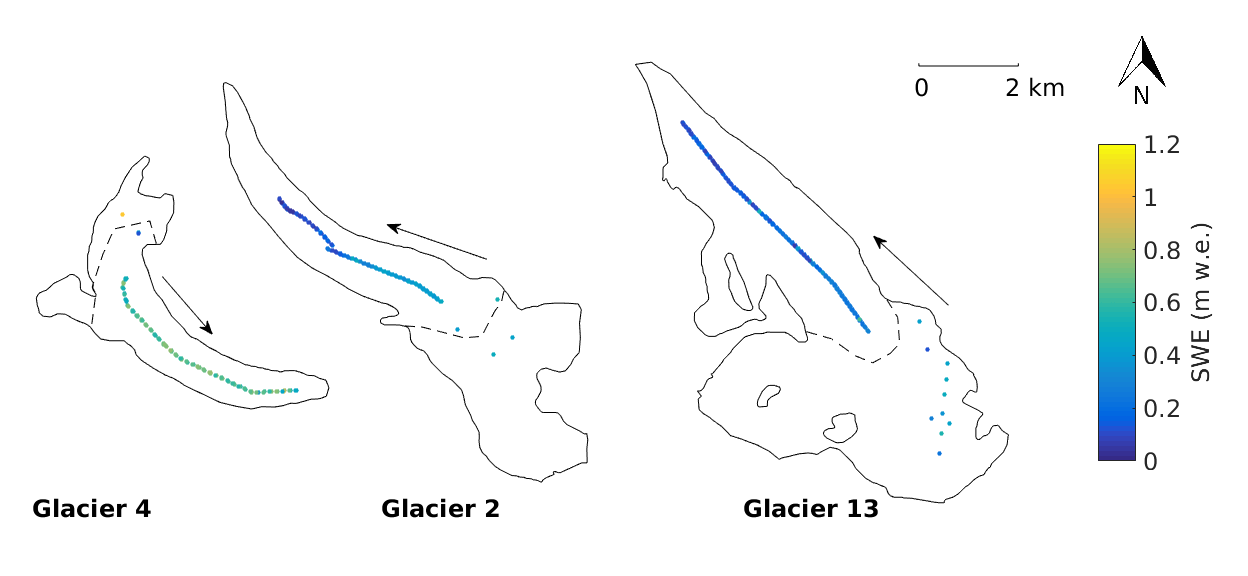
\includegraphics[width =\textwidth]{SamplingDesign_Acentreline.png}\\
	\caption{Centreline sampling design with accumulation area points as a subset of all measured locations. Dashed line is the approximate location of the ELA and arrow shows glacier flow direction.}
	\label{fig:SamplingDesign_Acentreline}
\end{figure}

\begin{figure}[H]
	\centering
	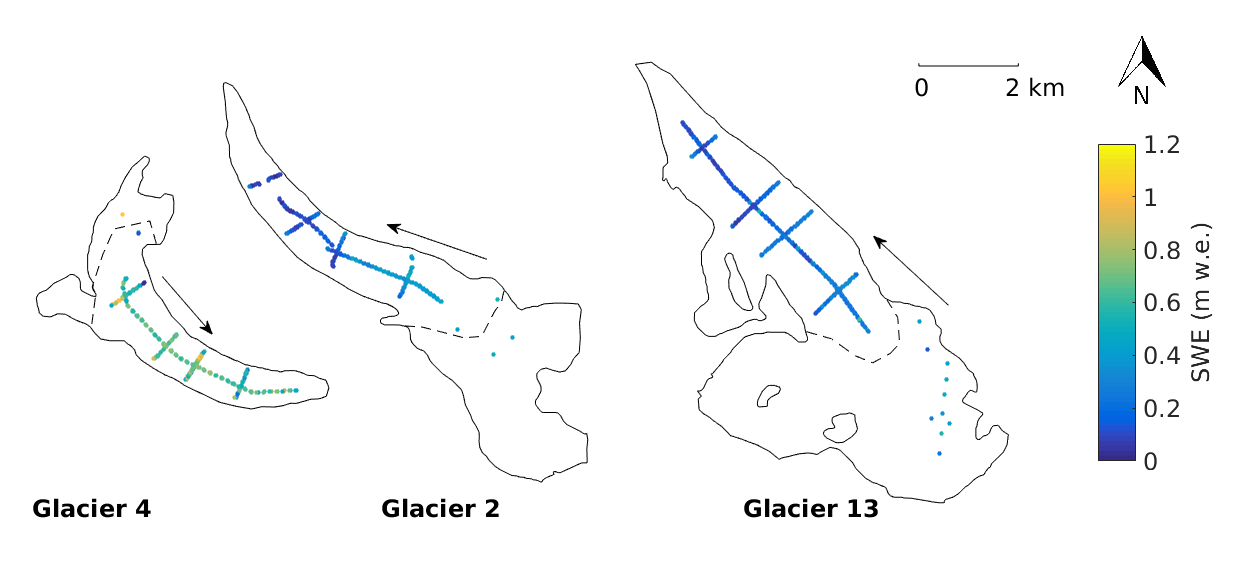
\includegraphics[width =\textwidth]{SamplingDesign_ACentreTransect4.png}\\
	\caption{Centreline and four transects sampling design with accumulation area points  as a subset of all measured locations. Dashed line is the approximate location of the ELA and arrow shows glacier flow direction.}
	\label{fig:SamplingDesign_ACentreTransect4}
\end{figure}

\begin{figure}[H]
	\centering
	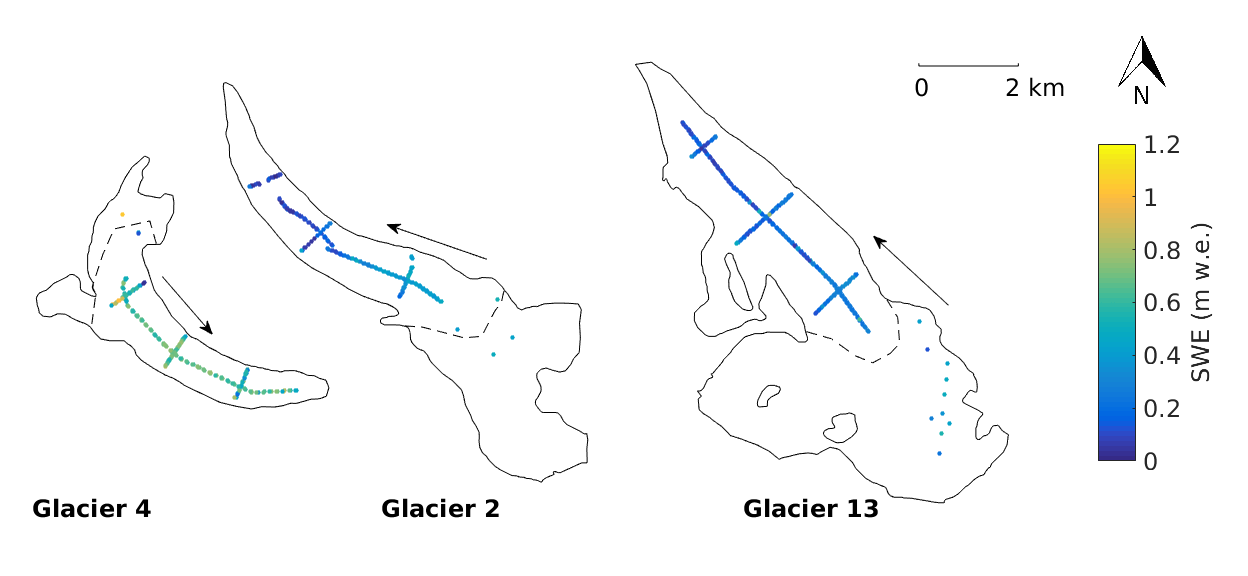
\includegraphics[width =\textwidth]{SamplingDesign_ACentreTransect3.png}\\
	\caption{Centreline and three transects sampling design with accumulation area points  as a subset of all measured locations. Dashed line is the approximate location of the ELA and arrow shows glacier flow direction.}
	\label{fig:SamplingDesign_ACentreTransect3}
\end{figure}

\begin{figure}[H]
	\centering
	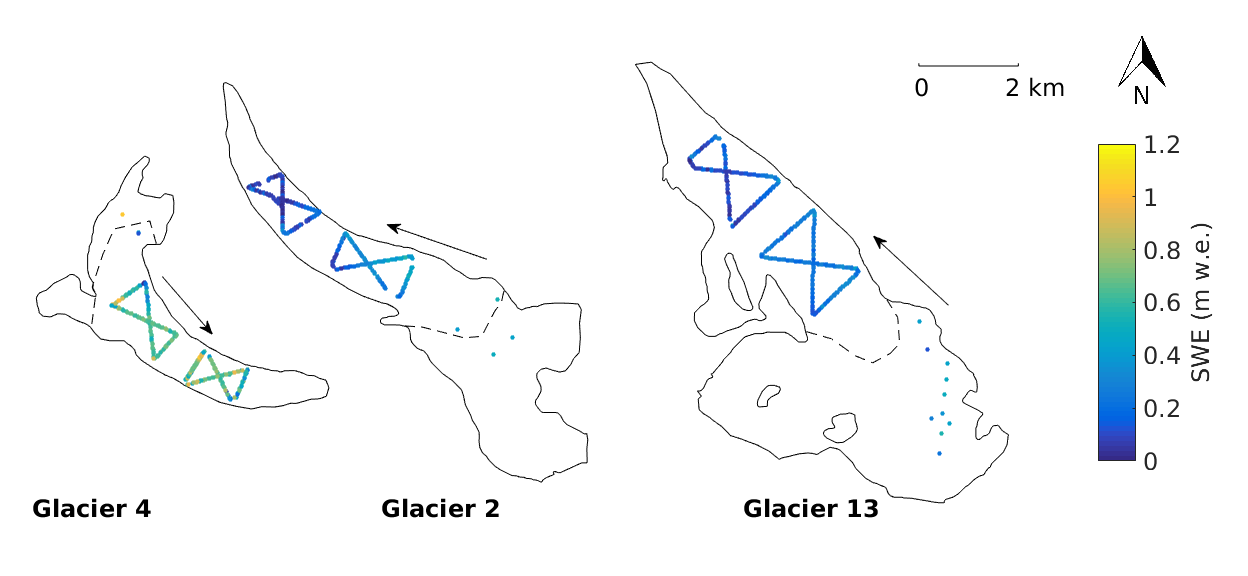
\includegraphics[width =\textwidth]{SamplingDesign_Ahourglass.png}\\
	\caption{Hourglass sampling design with accumulation area points as a subset of all measured locations. Dashed line is the approximate location of the ELA and arrow shows glacier flow direction.}
	\label{fig:SamplingDesign_Ahourglass}
\end{figure}

\begin{figure}[H]
	\centering
	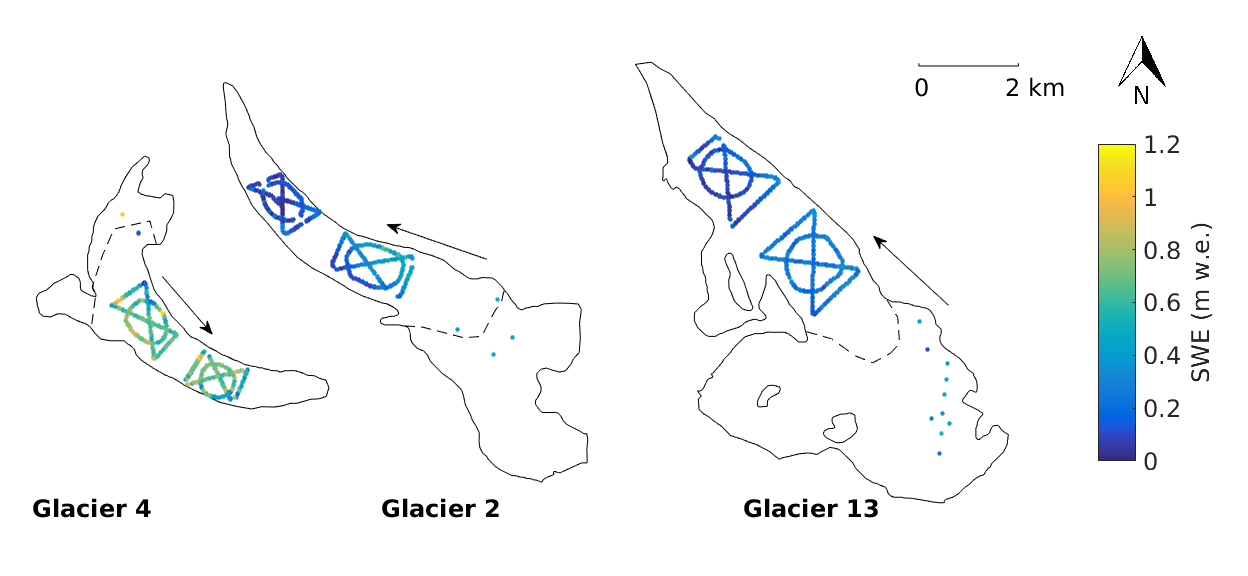
\includegraphics[width =\textwidth]{SamplingDesign_AhourglassCircle.png}\\
	\caption{Hourglass and circle sampling design with accumulation area points as a subset of all measured locations. Dashed line is the approximate location of the ELA and arrow shows glacier flow direction.}
	\label{fig:SamplingDesign_AhourglassCircle}
\end{figure}

	
	


\subsection{Results}

\pagebreak
\begin{figure}[H]
	\centering
	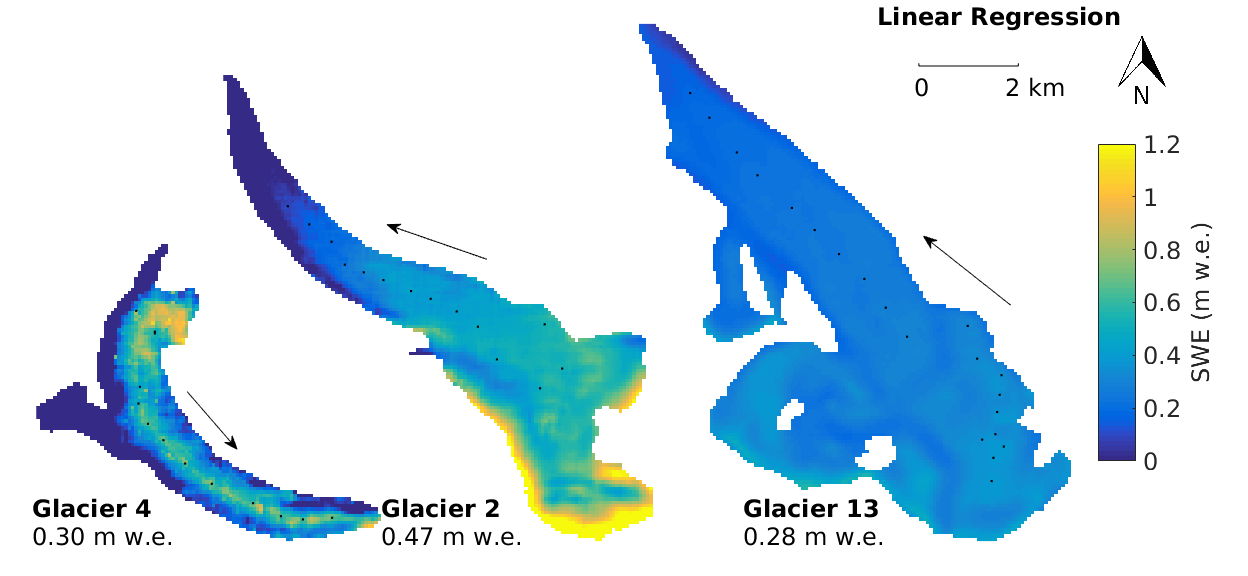
\includegraphics[width =0.9\textwidth]{MapSubset_LRcentreline_n10S4.png}\\
	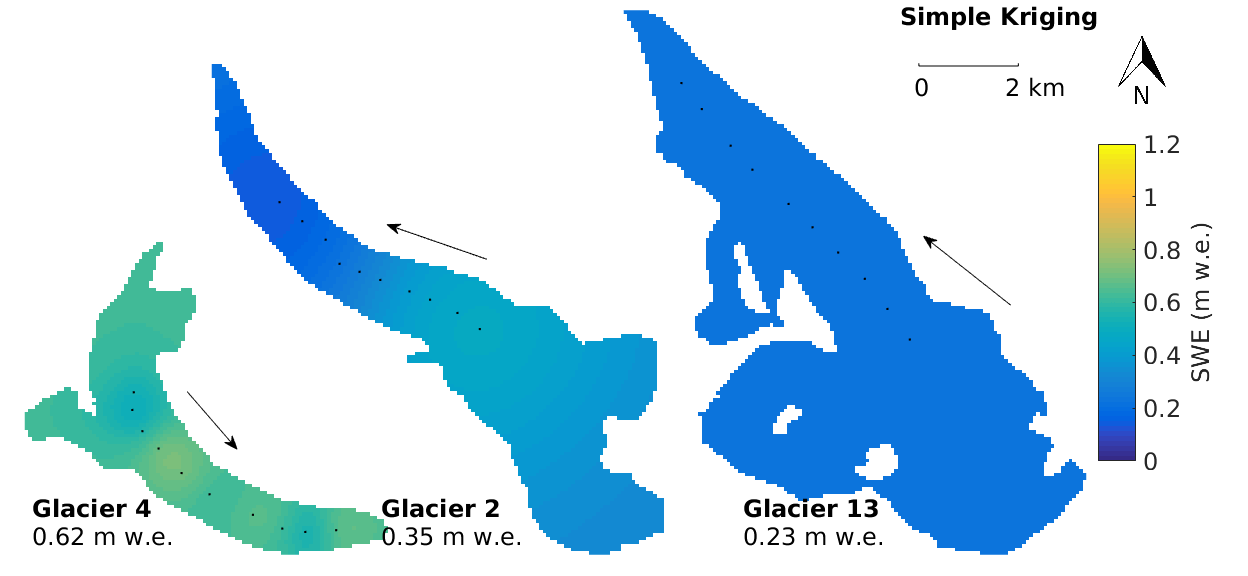
\includegraphics[width =0.9\textwidth]{MapSubset_SKcentreline_n10S4.png}\\
	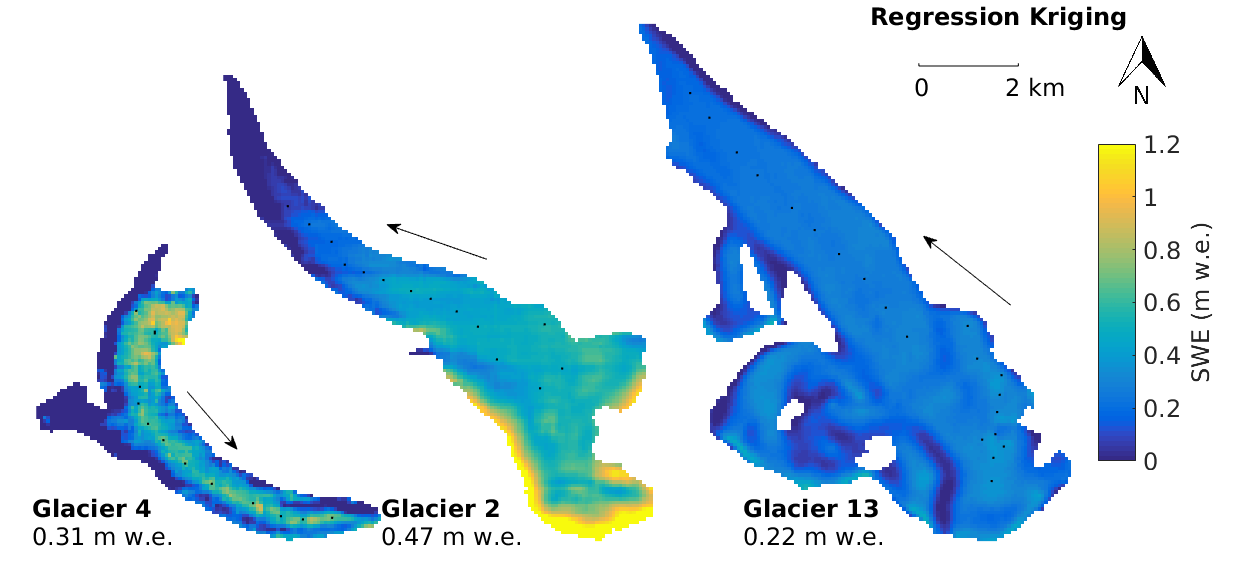
\includegraphics[width =0.9\textwidth]{MapSubset_RKcentreline_n10S4.png}\\
	\caption{Distributed winter surface mass balance found using  linear regression (MLR) (top), simple kriging (middle) and regression kriging (BMA) (bottom) on centreline subset data ($n=10$).  \topomap}
	\label{fig:MapSubset_centreline_n10S4}
\end{figure}


Based on RMSE
- LR sample size of 50 for G13 deffs, G2 pretty good

- G13 needs ~30 sample size regardless of interpolation (cf RK centreline wo accum)
- G4 centreline is garbage 

- RK sample size of 40-50 for all G generally good
- RK has lower RMSE (cf centreline)
- density affects it

- SK density has larger impact 
- sample size less of an impact (cf G13 usually has reduction of error at 40 points)

- centreline worst when linear regression used (not too bad for SK)
- hourglass has lowest RMSE (though no significant I image) on G2 and G13 (better than HGwC)
- CT4 better than CT3 but not by much

- generally, if you had accumulation points it's better but not a huge amount -> sometimes better to have a different design and no accum than another design and accum (e.g. G2 RK 

Based on SWE
- sample size doesn't really have effect
- kriging sampling design has little effect

%%%%%%%%%%%%%%%%%%%%%
\bibliography{/home/glaciology1/Documents/MastersDocuments/MastersLit}
\bibliographystyle{igs}
%%%%%%%%%%%%%%%%%%%%%

\section*{APPENDIX - Experimental design software}
\label{app:Subsets}
The experimental design component of this study examines the estimated WSMB using data subsets. Subsets are chosen based on the survey design component (e.g. centreline, hourglass) and a chosen sample size. Then, LR, SK and RK are used to find a glacier-wide distribution of SWE. This process is completed in the MATLAB script `BalanceDesign.m'. 
\begin{enumerate}
\item SWE values at all measurement locations are estimated using one of the density options (S1, F1, S2, F2, S3, F3, S4, F4).
\item The author-made function `DataSubset.m' is used to select all points that are a part of the chosen design subset (e.g. centreline, hourglass, etc.). The selection is made based on the sampling point classification that was determined in the sampling design (Sections \ref{sec:FieldDesign}). For example, only points that are classified as `UM' and `LM' are included in the `centreline' subset. Measurement locations that happen to fall along on the centreline but are a part of another sampling design subset, such as the hourglass, are not included. The corresponding topographic parameter values for each sampling subset location are then selected. 
\item The author-made function `ObsInCell.m' then takes the average SWE value of multiple measurement values within a single DEM cell. The result is one SWE value with a set of topographic parameters for each DEM cell where subset measurements are available.
\item Then, the author-made function `SortNSelect.m' orders the data by the cell number (origin at NW corner of DEM and increasing in the eastward and southward directions) and selects $n$ number of between the first and last point. The data are selected based on an equally spaced index vector that spans the length of the subset, not on the actual location of the data points, because data were collected in equally spaced intervals along a subset transect. The number of points ranged from 10 to 100 in increments of 10 for all subsets, expect for centreline subset where the range was from 10 to 50 points in increments of 5 points because of small subset length. 
\item Estimation of distributed SWE is then completed using the author-made functions `LinearRegression.m' for linear regression (LR), `KrigingR\_G.m' for simple kriging (SK) and `RegressionKriging.m' for regression kriging (RK). Each function uses its respective interpolation method to calculate a distributed SWE field and returns regression coefficients for LR and RK. 
\end{enumerate}

\end{document} 